
\documentclass[12pt]{amsart}   % LaTeX with AMS style; 12 point for old eyes

\usepackage{amsmath,amssymb,amsfonts}   % For better support of math
\usepackage{graphicx}	        % Enable for eps and pdf figures, if they occur
\usepackage{hyperref} % Enable embedded hyperlinks.
\hypersetup{
	hidelinks, colorlinks, linkcolor=black, citecolor=black, urlcolor=red
}
        
% Commands to force sequential numbering:

\newtheorem{theorem}{Theorem}[section]
\newtheorem{proposition}[theorem]{Proposition}
\newtheorem{lemma}[theorem]{Lemma}
\newtheorem{definition}[theorem]{Definition}
\newtheorem{examples}[theorem]{Examples}
\newtheorem{remarks}[theorem]{Remarks}
\newtheorem{corollary}[theorem]{Corollary}
\newtheorem{remark}[theorem]{Remark}
\newtheorem{example}[theorem]{Example}
\newtheorem{conjecture}[theorem]{Conjecture}

% Define abs norm, paren, bracket, cbracket, and innerproduct
\usepackage{mathtools}
\DeclarePairedDelimiter\tempabs{\lvert}{\rvert}
\DeclarePairedDelimiter\tempnorm{\lVert}{\rVert}
\DeclarePairedDelimiter\tempinnerproduct{\langle}{\rangle}
\DeclarePairedDelimiter\tempparen{(}{)}
\DeclarePairedDelimiter\tempbracket{[}{]}
\DeclarePairedDelimiter\tempcbracket{\{}{\}}

% Swap * functionality
\makeatletter
\def\abs{\@ifstar{\tempabs}{\tempabs*}}
\def\norm{\@ifstar{\tempnorm}{\tempnorm*}}
\def\innerproduct{\@ifstar{\tempinnerproduct}{\tempinnerproduct*}}
\def\paren{\@ifstar{\tempparen}{\tempparen*}}
\def\bracket{\@ifstar{\tempbracket}{\tempbracket*}}
\def\cbracket{\@ifstar{\tempcbracket}{\tempcbracket*}}
\makeatother

\graphicspath{ {figures/} }

\begin{document}

\title[The 18.821 report]{The 18.821 Mathematics Project Lab Report 
[Proofs]} 
% the first [...] gives a brief version of the title, which is long!
 
\author{Jonathan Allen}
\date{\today}              % or an actual date


\newcommand{\C}{\mathbb C} % blackboard bold , for ``complex,'' etc
\newcommand{\R}{\mathbb R} 
\newcommand{\Z}{\mathbb Z}
\newcommand{\Q}{\mathbb Q}
\newcommand{\N}{\mathbb N}

\maketitle

\section{Theorems}

\subsection{Notation\label{sec:notation}} 

\begin{description}
    \item[$t$] Time
    \item[$l(t)$] Path length
    \item[$s(t)$] Speed
    \item[$a_t(t)$] Tangential acceleration
    \item[$a_c(t)$] Centripetal acceleration
    \item[$\vec{x}(t)$] Position
    \item[$\vec{v}(t)$] Velocity
    \item[$\vec{a}(t)$] Acceleration
\end{description}

\section{Coordinate Systems}

\begin{align}
\dot{a}& = \frac{da}{dt}
\end{align}

\subsection{Rectangular Coordinates}


\begin{align}
R& = \abs{\frac{\paren{\dot{x}^2 + \dot{y}^2}^{3/2}}{\dot{x}\ddot{y} - \dot{y}{\ddot{x}}}}\\
%
&= \abs{\frac{s^2}{a_t}}\tag{for $a_c = $}
\end{align}

\subsection{Scalar Calculus in Polar Coordinates}

\begin{align}
s& = \frac{dl}{dt}\\
%
a_t& = \frac{ds}{dt}\\
\end{align}

\subsection{Vector Calculus in Polar Coordinates}

\begin{align}
\boldsymbol{x}& = r \boldsymbol{\hat{r}}\\
%
\boldsymbol{\vec{v}}& = \dot{r} \boldsymbol{\hat{r}} + r \dot{\phi} \boldsymbol{\hat{\phi}}\\
%
\label{eq:a_vec_def}\boldsymbol{\vec{a}}& = \paren{\ddot{r} - r \dot{\phi}^2} \boldsymbol{\hat{r}} + \frac{1}{r} \frac{d}{dt} \paren{r^2 \dot{\phi}} \boldsymbol{\hat{\phi}}
\end{align}

\subsection{Relations}

\begin{align}
l& = \int_{t=0}^{T} \norm{\boldsymbol{\vec{v}} \, } \; dt\\
%
s& = \norm{\boldsymbol{\vec{v}}}\\
%
a_t& = \norm{\boldsymbol{\vec{a}}} \cdot \boldsymbol{\hat{v}} = \norm{\boldsymbol{\vec{a}}} \cdot \frac{\boldsymbol{\vec{v}}}{\norm{\boldsymbol{\vec{v}}}}\\
%
a_c& = \norm{\boldsymbol{\vec{a}}} \times \boldsymbol{\hat{v}} = \norm{\boldsymbol{\vec{a}}} \times \frac{\boldsymbol{\vec{v}}}{\norm{\boldsymbol{\vec{v}}}}
\end{align}

\section{Lemmas and Definitions}

\begin{lemma}
If $a_t=0$ and $\norm{a_c} \le a_{c,max}$, then the minimum radius of curvature of a point trajectory is given by
\begin{equation}
R_{min} = \frac{v^2}{a_{c,max}}
\end{equation}
\end{lemma}

\proof 

\begin{figure}
\begin{center}
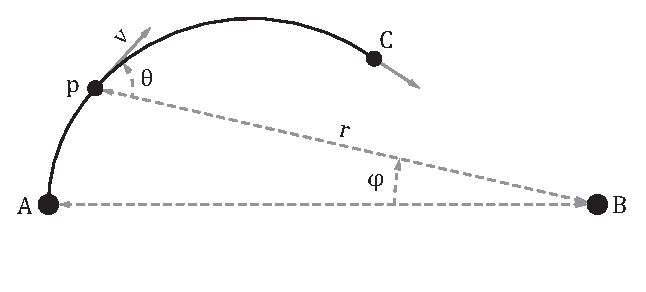
\includegraphics[width=4in]{arc_param.eps}
\end{center}
\vspace{-.2in} % corrects bad spacing
\caption{My first .eps figure.\label{fig:2}}
\end{figure}

If we look at a position, p, on a trajectory. We can align a rectangular coordinate system with this point, such that $\hat{y} = \hat{v}$.

\begin{align}
a_c& = \ddot{r} - r \dot{\phi}^2\\
%
a_t& = \frac{1}{r} \frac{d}{dt} \paren{r^2 \dot{\phi}}\\
%
0& = \frac{1}{r} \frac{d}{dt} \paren{r^2 \dot{\phi}}\\
%
r^2 \dot{\phi}& = constant
\end{align}

\qed

\section{Theorems}

\begin{theorem}
If $a_t=0$ and $\norm{a_c} \le a_{c,max}$, it is always optimal to minimize the turning radius.
\end{theorem}

\proof

\begin{align}
\boldsymbol{\vec{v}}& = \dot{r} \boldsymbol{\hat{r}} + r \dot{\phi} \boldsymbol{\hat{\phi}}\\
%
s& = \sqrt{\dot{r}^2 + r^2 \dot{\phi}^2}\\
%
\dot{r}& = s^2 - r^2 \dot{\phi}^2
\end{align}

\qed

\bibliographystyle{plain}
\begin{thebibliography}{9}
\bibitem{wiki_pcoords}
\url{http://en.wikipedia.org/wiki/Polar_coordinate_system}
\end{thebibliography}

\end{document}

From Spring 2011 or before; revised by Miller, Spring 2013. 
